%----------------------------------------------------------------------------------------
%
% A LaTeX-template for 1DV510. Modified and translated by Björn Lindenberg at LNU.
% Based on an original master thesis template created by Marcus Wilhelmsson at LNU.
%
%----------------------------------------------------------------------------------------

% Settings and document configuration

\documentclass[a4paper,12pt]{article} 
\usepackage[T1]{fontenc} 
\usepackage{times} 
\usepackage[swedish,english]{babel} 
\usepackage[utf8]{inputenc} 
\usepackage{dtk-logos} 
\usepackage{wallpaper} 
\usepackage[absolute]{textpos} 
\usepackage[top=2cm, bottom=2.5cm, left=3cm, right=3cm]{geometry} 
\usepackage[parfill]{parskip} 
\usepackage{csquotes} 
\usepackage{float} 
\usepackage{lipsum} % Used for dummy text. Can be removed.
\usepackage{listings, color}

\lstdefinestyle{Asm}{
  belowcaptionskip=1\baselineskip,
  breaklines=true,
  frame=L,
  xleftmargin=\parindent,
  language=[x86masm]Assembler,
  showstringspaces=false,
  basicstyle=\footnotesize\ttfamily,
  keywordstyle=\bfseries\color{purple!40!black},
  commentstyle=\itshape\color{green!40!black},
  identifierstyle=\color{blue},
  stringstyle=\color{orange},
}

% Fontsizes for section headings.
\usepackage{sectsty} 
\sectionfont{\fontsize{14}{15}\selectfont}
\subsectionfont{\fontsize{12}{15}\selectfont}
\subsubsectionfont{\fontsize{12}{15}\selectfont}

%----------------------------------------------------------------------------------------
%	This part is used for the text box on the title page
%----------------------------------------------------------------------------------------
\newsavebox{\mybox}
\newlength{\mydepth}
\newlength{\myheight}

\newenvironment{sidebar}%
{\begin{lrbox}{\mybox}\begin{minipage}{\textwidth}}%
{\end{minipage}\end{lrbox}%
 \settodepth{\mydepth}{\usebox{\mybox}}%
 \settoheight{\myheight}{\usebox{\mybox}}%
 \addtolength{\myheight}{\mydepth}%
 \noindent\makebox[0pt]{\hspace{-20pt}\rule[-\mydepth]{1pt}{\myheight}}%
 \usebox{\mybox}}

%----------------------------------------------------------------------------------------
%	Title
%----------------------------------------------------------------------------------------
\newcommand\BackgroundPic{
    \put(-2,-3){
    
\includegraphics[keepaspectratio,scale=0.3]{img/lnu_etch.png} % Background image
    }
}
\newcommand\BackgroundPicLogo{
    \put(30,740){
    
\includegraphics[keepaspectratio,scale=0.10]{img/logo.png} % LNU logo
    }
}

\title{
\vspace{-8cm}
\begin{sidebar}
    \vspace{10cm}
    \normalfont \normalsize
    \huge Computer Technology I\\ % Main title
    \vspace{-1.3cm}
\end{sidebar}
\vspace{3cm}
\begin{flushleft}
    \huge Lab. 6: CyberTech Wall Display % Subtitle
     \small \\ \emph{}
\end{flushleft}
\null
\vfill
\begin{textblock}{5}(10,13)
\begin{flushright}
\begin{minipage}{\textwidth}
\begin{flushleft} \large
\emph{Author:}\textsc{ Loic GALLAND, Leonardo PEDRO}\\  % Author
\emph{Supervisor:}  \textsc{} \\  % Author
\emph{Semester:} Autumn 2019\\ % Semester
\emph{Area:} Computer Science \\ % Area
\emph{Course code:} 1DT301 % Course
\end{flushleft}
\end{minipage}
\end{flushright}
\end{textblock}
}

\date{} % Empty date command. Use \today inside for today's date.
\author{} % Normally one would use this to define authors. However in this case the title command takes care of everything, so we leave the field empty to get rid of warnings. 

\begin{document}

\pagenumbering{gobble} % Turn off page numbering
\newgeometry{left=5cm}
\AddToShipoutPicture*{\BackgroundPic} % Adds the background image to the title page
\AddToShipoutPicture*{\BackgroundPicLogo} % Adds the logo to the title page
\maketitle % Prints the title
\restoregeometry
\clearpage

\pagenumbering{roman} % Roman page numbering for abstract page


\selectlanguage{english}

\newpage

\pagenumbering{gobble} % Turn off page numbering
\tableofcontents 

\newpage
\pagenumbering{arabic} % Turn on page numbering


\section{Task 1 - Write a program that writes a character on the CyberTech Display}

\textit{Any character can be displayed. The display is connected to the serial port (RS232) on the
STK600. Communication speed is 2400 bps. 
}

\lstset{style=Asm}
\begin{lstlisting}
;>>>>>>>>>>>>>>>>>>>>>>>>>>>>>>>>>>>>>>>>>>>>>>>>>>>>>>>>>>>
; 1DT301, Computer Technology I
; Date: 2019-10-20
; Author:
; Loic GALLAND
; Leonardo PEDRO
;
; Lab number: 6
; Title: CyberTech Wall Display
;
; Hardware: STK600, CPU ATmega2560
;
; Function: Write a program that writes a character on the CyberTech Display
;			
; Input ports: Port0 (RS232) VGA 
;
; Output ports: Port0 (RS232) VGA
;
; Subroutines: If applicable.
; Included files: m2560def.inc
;<<<<<<<<<<<<<<<<<<<<<<<<<<<<<<<<<<<<<<<<<<<<<<<<<<<<<<<<<<<

#include <avr/io.h>
#include <stdio.h>
#include <string.h>
#define F_CPU 1843200 //Clock Speed
#define BAUD 2400
#define MYUBRR (F_CPU/16/BAUD-1)

void USART_Unit(unsigned int ubrr);
void toPutty(unsigned char data);

int main(void)
{
	USART_Unit(MYUBRR);
	char* temp = "\rAO0001LOIC&LEO"; //Begiining code to send to the display + actual text.
	int length = 15;
	int checksum = 0;
	
	;Use checksum to make sure that what was sent and was received is the same.
	for (int i=0;i<strlen(temp);i++ )
	{
		checksum+=temp[i];
	}
	
	checksum%=256;
	
	char toPrint[strlen(temp)+3];
	
	sprintf(toPrint,"%s%02X\n",temp,checksum);
	
	for(int j=0;j<length+4;j++){
		toPutty(toPrint[j]);
	}
	
	temp = "\rZD0013C\n";//End code to be sent to the display to say that what needed to be sent has been sent.
	
	for (int k=0;k<strlen(temp);k++)
	{
		toPutty(temp[k]);
	}
	
}
;TO INITIALIZE THE USART CONNECTION
void USART_Unit(unsigned int ubrr){
	UBRR1L = ubrr;
	
	;/*	Enable receiver and transmitter	*/
	UCSR1B = (1<<RXEN1)|(1<<TXEN1);
}

;To send to the the display the character
void toPutty(unsigned char data){
	; Wait for data to be received
	while ( !(UCSR1A & (1 << UDRE1))); //Receive Complete
	;RXCn) flag //Return received data from buffer
	UDR1 = data;
}
\end{lstlisting}
\newpage
This is the flowchart of the task 1:
\begin{center}
%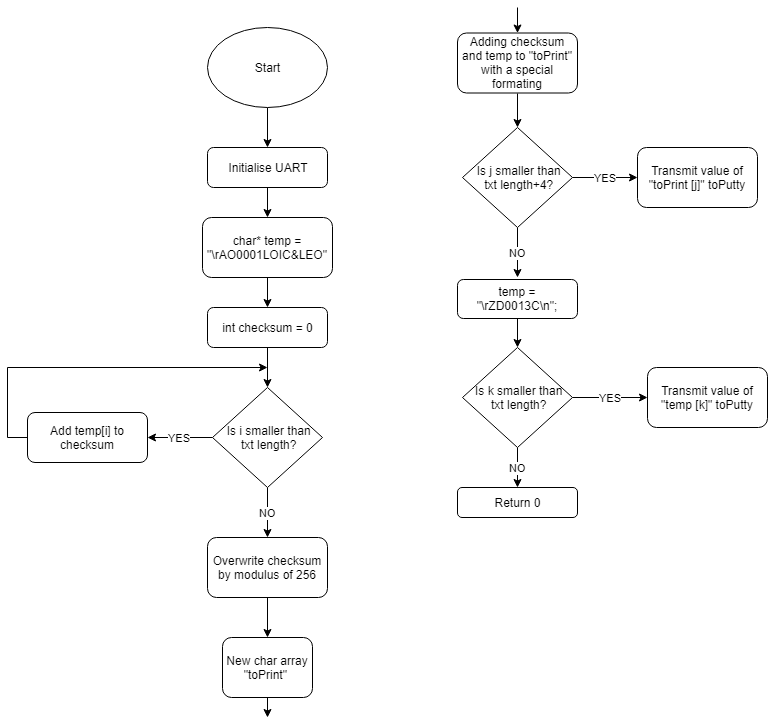
\includegraphics[scale=0.8]{img/Task1.png}
\end{center}
\newpage
\section{Task 2 - Write a program that writes characters on all text-lines on the CyberTech Display}
\textit{The program will write to all three rows.}

\lstset{style=Asm}
\begin{lstlisting}
;>>>>>>>>>>>>>>>>>>>>>>>>>>>>>>>>>>>>>>>>>>>>>>>>>>>>>>>>>>>
; 1DT301, Computer Technology I
; Date: 2019-10-20
; Author:
; Loic GALLAND
; Leonardo PEDRO
;
; Lab number: 6
; Title: CyberTech Wall Display
;
; Hardware: STK600, CPU ATmega2560
;
; Function: Write a program that writes characters on all text-lines on the CyberTech
;			Display. 
;			
; Input ports: Port0 (RS232) VGA 
;
; Output ports: Port0 (RS232) VGA
;
; Subroutines: If applicable.
; Included files: m2560def.inc
;<<<<<<<<<<<<<<<<<<<<<<<<<<<<<<<<<<<<<<<<<<<<<<<<<<<<<<<<<<<
#include <avr/io.h>
#include <stdio.h>
#include <string.h>
#define FCPU 1000000// Clock Speed
#define BAUD 2400 //Communication Speed Display rate 2400
#define MYUBBRR (FCPU/16/BAUD-1) ;UBBRR = 25 -> osc = 1MHz

void uart_int(void);
void toPutty(unsigned char data);
void toDisplayOnLCD(char* stringChar);

int main(void)
{
	uart_int();
	
	char* txt = "\rAO0001First Line              Second Line";
	
	toDisplayOnLCD(txt);
	
	txt = "\rBO0001Third Line"; //Begining combination for the third line
	toDisplayOnLCD(txt);
	
	txt = "\rZD0013C\n"; //Ending combination to tell the display everything been sent.
	toDisplayOnLCD(txt);
	
	return 0;
}

void toDisplayOnLCD(char* stringChar){
	
	int checksum = 0;
	
	for(int i =0; i<strlen(stringChar);i++){
		checksum += stringChar[i];
	}
	
	checksum%=256;
	
	char toDisplay [strlen(stringChar)+3];
	sprintf(toDisplay, "%s%02X\n", stringChar, checksum); //%02x means print at least 2 digits, prepends it with 0's if there's less.
	;%02x is used to convert one character to a hexadecimal string
	
	for (int i = 0; i<strlen(stringChar)+3;i++){
		toPutty(toDisplay[i]);
	}
}

void toPutty(unsigned char data){

	while(!(UCSR1A & (1<<UDRE1)));
	UDR1 = data;
}

void uart_int(void) {
	UBRR1L = MYUBBRR; //25 because we are setting the board at 1MHz
	
	UCSR1B = (1<<RXEN1|1<<TXEN1); // Enable receive and transmit bit
}
\end{lstlisting}
\newpage
This is the flowcharts of the task 2:
\begin{center}
%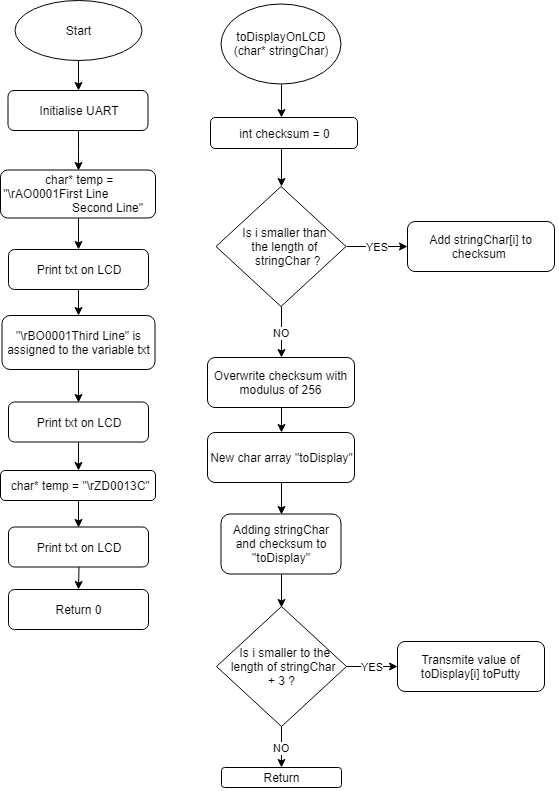
\includegraphics[scale=0.9]{img/Task2.png}
\end{center}

\newpage
\section{Task 3 -Write a program that change text strings on the display}
\lstset{style=Asm}
\begin{lstlisting}
;>>>>>>>>>>>>>>>>>>>>>>>>>>>>>>>>>>>>>>>>>>>>>>>>>>>>>>>>>>>
; 1DT301, Computer Technology I
; Date: 2019-10-20
; Author:
; Loic GALLAND
; Leonardo PEDRO
;
; Lab number: 6
; Title: CyberTech Wall Display
;
; Hardware: STK600, CPU ATmega2560
;
; Function: Write a program that change text strings on the display. 
;			
; Input ports: Port0 (RS232) VGA 
;
; Output ports: Port0 (RS232) VGA
;
; Subroutines: If applicable.
; Included files: m2560def.inc
;<<<<<<<<<<<<<<<<<<<<<<<<<<<<<<<<<<<<<<<<<<<<<<<<<<<<<<<<<<<

#include <avr/io.h>
#include <stdio.h>
#include <string.h>
#include <stdlib.h>

#define ClockSpeed 1000000 ;Clock Speed
#include <util/delay.h>
#define BAUD 2400 ;Communication Speed Display rate 2400
#define MYUBBRR (ClockSpeed/16/BAUD-1) ;UBBRR = 25 -> osc = 1MHz

void uart_int(void);
void toPutty(unsigned char);
void toDisplayOnLCD(char*);


void  toDisplayOnLCD(char* character){  ;Showing data into the big display
	
	int checksum = 0;
	
	for(int i =0;i<strlen(character);i++){
		checksum += character[i];
	}
	
	checksum%=256;
	
	char sendingToDisplay [strlen(character)+3];
	sprintf(sendingToDisplay, "%s%02X\n", character, checksum); //%02x means print at least 2 digits, prepends it with 0's if there's less.
	;%02x is used to convert one character to a hexadecimal string
	
	for (int i = 0; i<strlen(character)+3;i++){
		toPutty(sendingToDisplay[i]);
	}
}

void toPutty(unsigned char data){
	while(!(UCSR1A & (1<<UDRE1)));
	UDR1 = data;
}

void uart_int(void) {
	UBRR1L = MYUBBRR; //25 --> board at 1MHz
	
	UCSR1B = (1<<RXEN1|1<<TXEN1); // Receive Enable (RXEN) bit // Transmit Enable (TXEN) bit
}

int main(void)
{
	uart_int();
	

	char* text = "abc";
	char* begin = "\rAO0001";
	
	for(int i =0;i<strlen(text);i++){ 	//Go through every character and add it to the string 
		char a = text[i];
		size_t length = strlen(begin);
		
		char* textToBeSent = malloc(length + 1 + 1); //Giving memory space to allocate the data to str2
		strcpy(textToBeSent, begin); // copy txt to str2
		
		textToBeSent[length] = a;  
		textToBeSent[length + 1] = '\0'; // adding the end char \0
		 toDisplayOnLCD(textToBeSent); 
		free(textToBeSent); // deallocate the memory space used by malloc()
		
		;Ending combination to tell the Display that everything was sent.
		textToBeSent = "\rZD0013C";
		 toDisplayOnLCD(textToBeSent);

		_delay_ms(4000); //wait 4s between each letter so that we actually have time to see the change.
	}

	
	return 0;
}
\end{lstlisting}
This is the flowchart of the task 3:
\begin{center}
%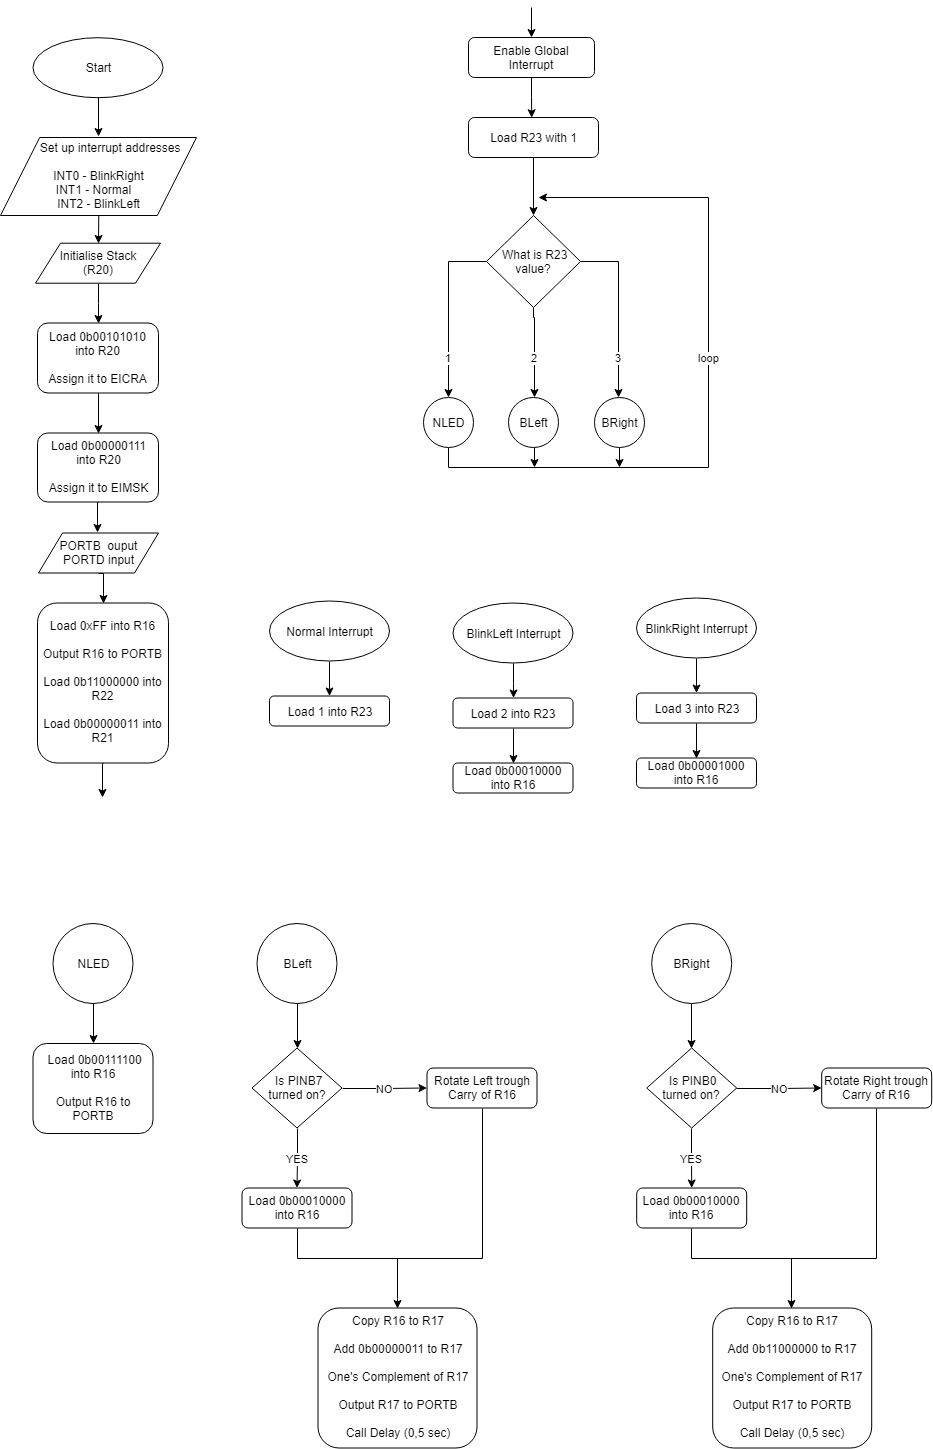
\includegraphics[scale=0.8]{img/TASK3.png}
\end{center}
\newpage
\section{Task 4 - Write a program that communicates with both the terminal and the display}
\textit{Since we only have one serial port, we must make a special cable, so that the STK600 receive unit
is connected to the terminal (PuTTY, for instance) and transmit is connected to the display. Text
can be entered at the terminal. End of line with a special character that you choose. It should also
be possible to enter address on the screen to display text.}

\lstset{style=Asm}
\begin{lstlisting}

#include <stdlib.h>
#include <stdio.h>
#include <string.h>
#include <avr/io.h>

#define Card_CPU 1000000 ;Clock Speed of the CPU

#define BAUDRATE 2400 ;Display rate of 2400
#define MY_UBBRR (Card_CPU/16/BAUDRATE-1) ;Baud Rate = 25 -> osc = 1MHz -> Display rate speed = 2400
#define Valid_Digits "123"
#define SELECT_LINE '>' ;Char for line selection
#define TOTAL_AMOUNT_CHARS	24
#define TOTAL_AMOUNT_LINES 3 ;change this to 8 for Task 5


int line = 0; //To keep track of the current line
char line_selection = 0;
char text[8][TOTAL_AMOUNT_CHARS] = { "", "", "", "", "", "", "", "" };

;Declaration of the differents methods that will be used
void toPutty(unsigned char);
void uart_int(void);
void line_switch(int);
char getChar();
char contains_character(char*, char);
void refresh_text(void);
void toSendToDisplay(char, char*, char*);


int main(void)
{
	uart_int(); //Method to initialize the display
	refresh_text();
	
	while (1) {
		;Get the input from PuTTY
		char input = getChar(); 

		
		if (line_selection) {;If the line selection is selected then do nothing and wait for a line number
			if (input < '1') {
				;if the input is lower than 1 than do nothing and wait for another input
				continue; 
			}
			;Check if the input is included in the valid digits if it is then go inside if otherwise skip the if statement
			if (contains_character(Valid_Digits, input)) {

				line_selection = 0;
				line_switch((input - '1')); // turn the input into sterile int
				
			}
		} ;if there is no line selection then the code goes here
		else {
			;if the input is equal to '>' then change the line_selection to 1 (true)
			if (input == SELECT_LINE){

				line_selection = 1;

			}else if (input == 13 ){ ;Otherwise if the input is the carriage return(ENTER) then switch line
			
				line_switch(-1);
			
			}else {
				;Otherwise add the character to the corresponding lane
				char* line = text[line];
				sprintf(line, "%s%c", line, input);
			}
		}
		;Update the screen with with the corresponding changes 
		refresh_text();
	}

	return 0;
}

//
void toPutty(unsigned char data){
	
	while(!(UCSR1A & (1<<UDRE1))){
		;Do nothing while no data has been sent
	}
	UDR1 = data; 
}

;To initialize the display
void uart_int(void) {
	UBRR1L = MY_UBBRR; //Set the Baud Rate to 25. 

	UCSR1B = (1<<RXEN1|1<<TXEN1); //Enable Receive and Transmit bit
}

char getChar(){
	
	while(!(UCSR1A & (1<<RXC1))){
		;While no data has been received, do nothing
	}
	return UDR1; //return the received char.
}


;//Method to send the characters to the Display
void toSendToDisplay(char address, char* command, char* message)
{
	; Get the lengths of the command characters and of the message
	int command_length = sizeof(command);
	int message_length = sizeof(message);

	; Calculate how big the buffer needs to be depending on the message, command. 
	int buffer_length = 1 + command_length + message_length + 3;

	;Will add the adress + command + message + checksum, together to then send it to the screen 
	char* buffer_message = malloc(buffer_length);

	;Create the buffer with all the info needed
	sprintf(buffer_message, "\r%c%s%s", address, command, message);

	;Checksum calculation 
	unsigned int checksum = 0;
	for (int i = 0; (buffer_message[i] != 0); i++){
		checksum += buffer_message[i];
	}
	
	
	checksum %= 256;

	;Add the checksum to the buffer
	sprintf(buffer_message, "%s%02X\n", buffer_message, checksum);

	
	for (int i = 0; buffer_message[i]; i++){
		toPutty(buffer_message[i]);
	}
	
	;To free the space from memory
	free(buffer_message); 
}

;Method to check if the char "character" is in the "string". If it is return 1 otherwise return 0.
char contains_character(char* string, char character)
{
	char t;
	while ((t = *string++)){
		if (t == character) {
			return 1;
		}
	}
	return 0;
}

;Method to change between each line. if "-1" is sent then it will change the line. 
void line_switch(int number)
{
	;if numver =-1 then increment the current line
	if (number == -1) {
		line++;
		if (line >= TOTAL_AMOUNT_LINES)
		line = 0;
	}else {
		line = number;
	}
	
}

;To update the text on the display
void refresh_text()
{
	;To have the line to display
	int lineToDisplay = line;
	if (lineToDisplay < 1){
	lineToDisplay++;
	}
	;variable to set up the first and second line 
	char memory_ligne1_2[48] = "";
	char line_selected = line_selection ? '_' : (line + '1');

	
	sprintf(memory_ligne1_2, "Choose line: %c          %s", line_selected, text[lineToDisplay-1]);

	;Creates the third ligne 
	char memory_ligne3[48] = " ";
	if (text[lineToDisplay][0]){ //if the character is "0" do nothing otherwise send to "toSendToDisplay"
		;DO nothing
	}else { 
		for (int i = 0; i < 48; i++){
			memory_ligne3[i] = text[lineToDisplay][i];
		}
	}
	; Updates all the lignes of the screen. 
	toSendToDisplay('A', "O0001", memory_ligne1_2);
	toSendToDisplay('B', "O0001", memory_ligne3);
	toSendToDisplay('Z', "D001", 0);
}

\end{lstlisting}

\newpage
This is the flowchart of the task 4:
\begin{center}
%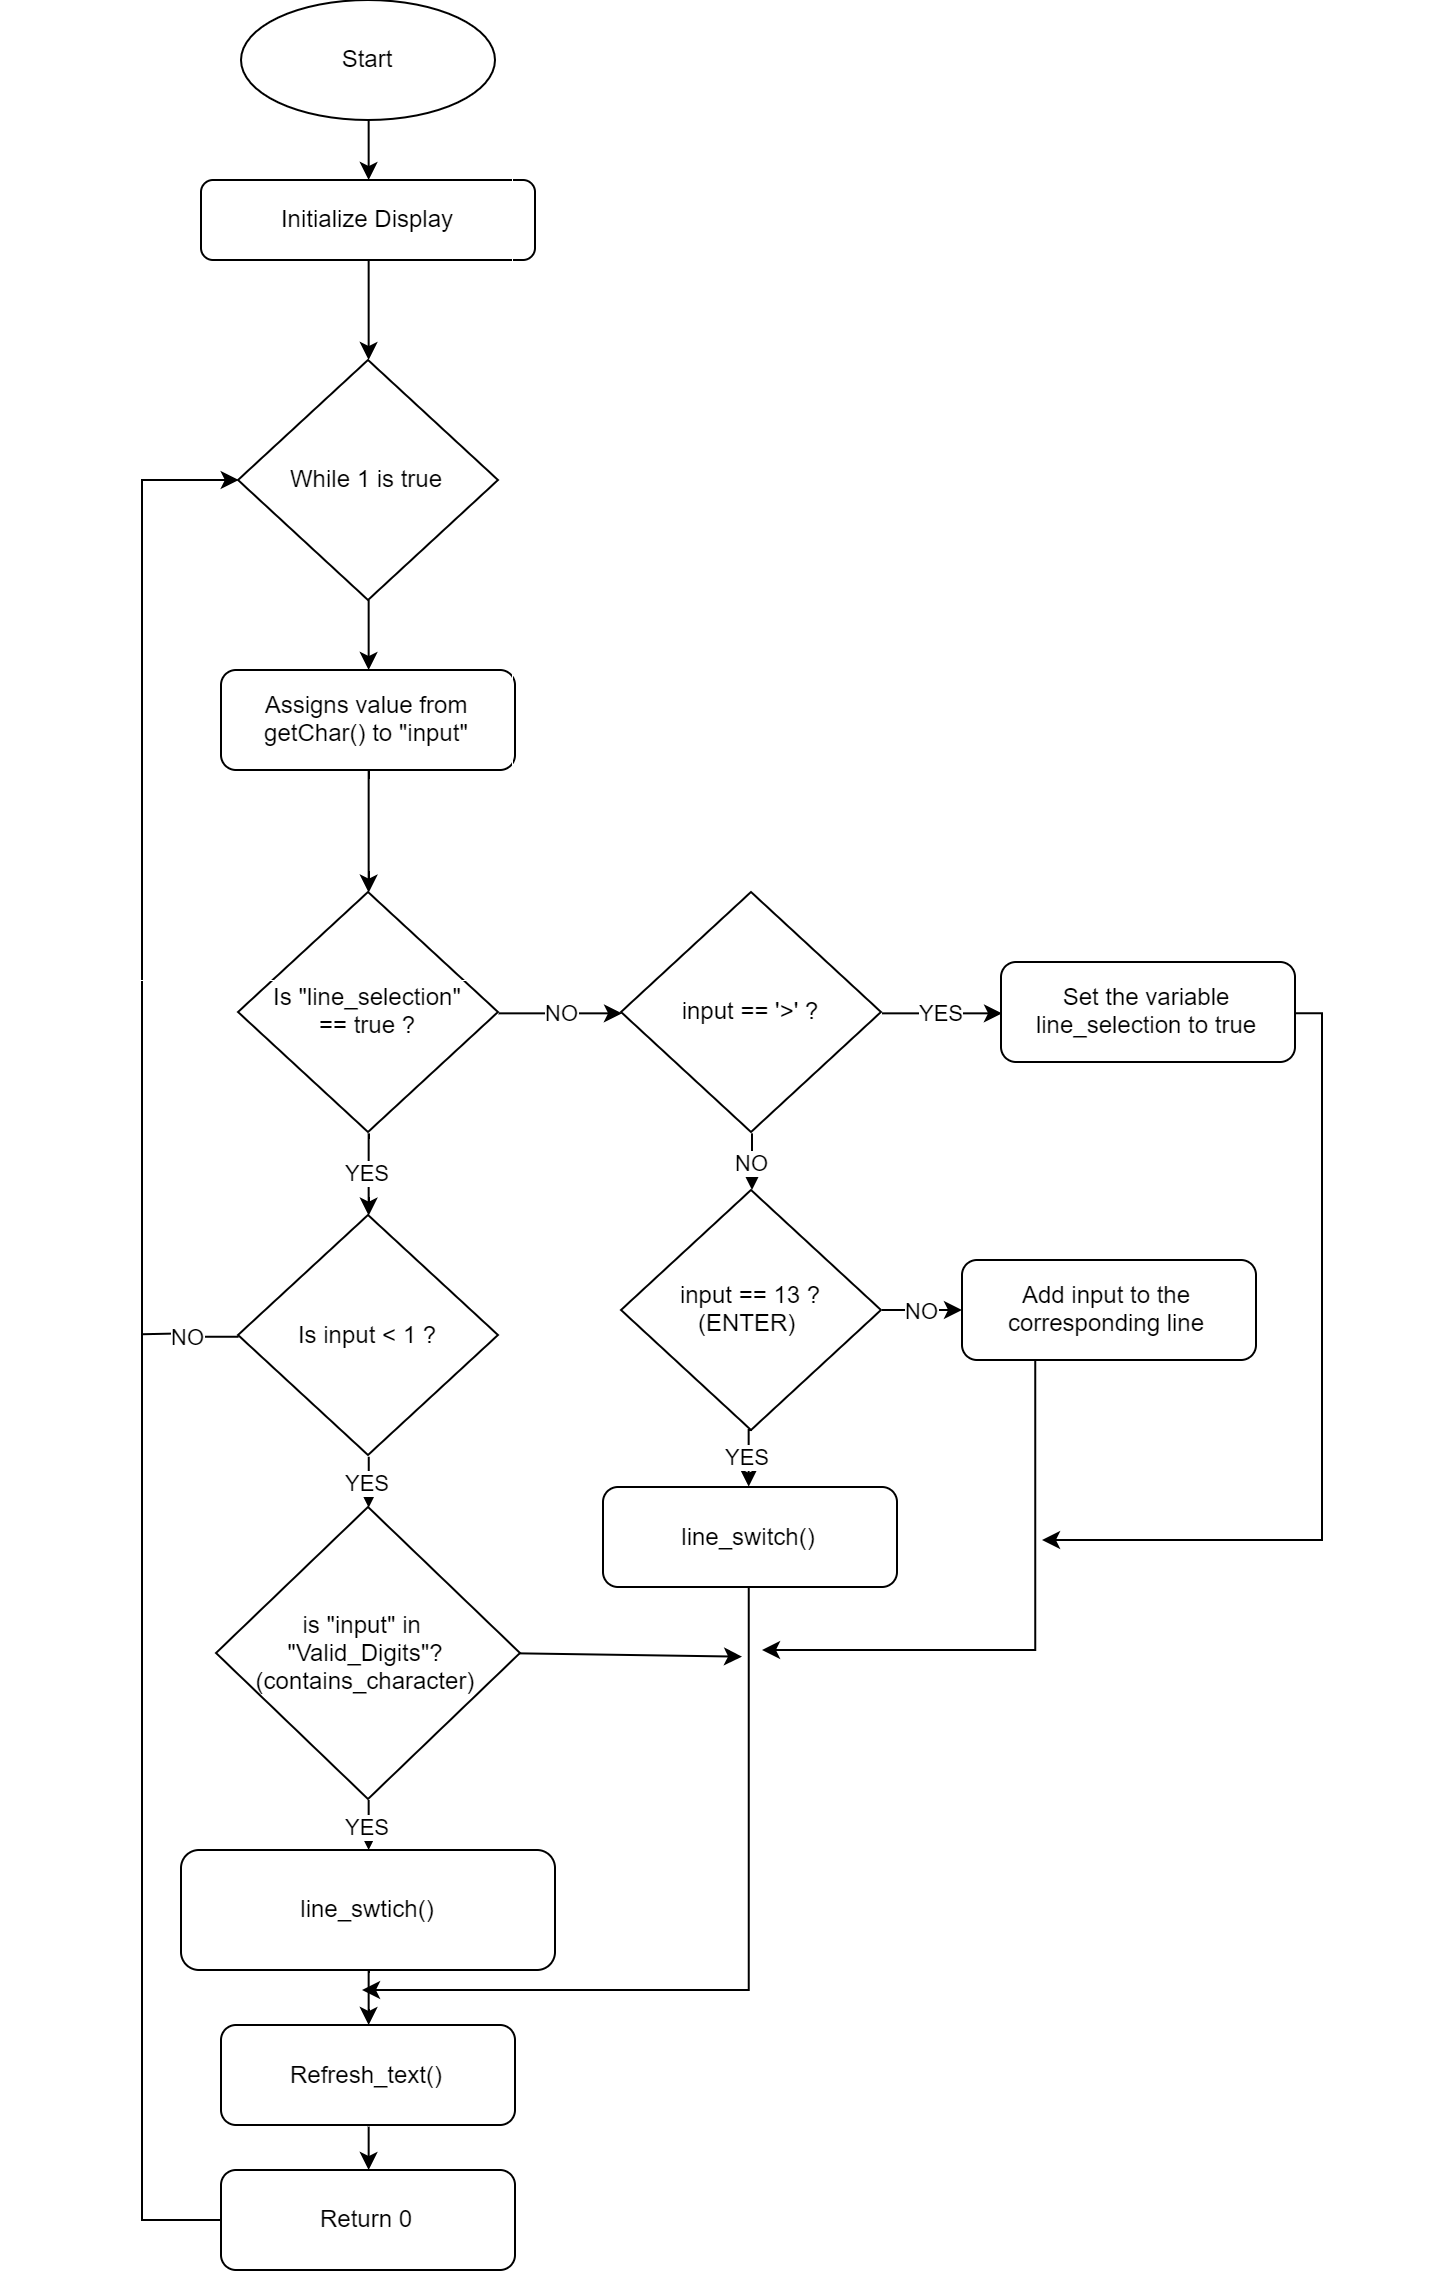
\includegraphics[scale=0.6]{img/Task4.png}
\end{center}
\newpage
\section{Task 5 - Write a program for text input. }
\textit{This exercise works exactly like Task 4. Therefore please refer to task 4.}

% Prints your bibliography database xxx.bib
\bibliographystyle{IEEEtran}
\bibliography{ref.bib}

\end{document}
